\documentclass[10pt,letterpaper]{article}

% -----------------------------------------------------------------------------
% Measuring What We Mean — position paper v8 (2026-08-10)
% Construct-identified inference: validate first, propagate second.
% Engine: cvprofiles 3.0.0 (released on PyPI 2026-08-10); accepted verifier-gated
% WVS/GPS patience application as initial real-data proof of work.
% -----------------------------------------------------------------------------
\usepackage[margin=0.88in,top=0.82in,bottom=0.82in]{geometry}
\usepackage{mathptmx}
\usepackage[T1]{fontenc}
\usepackage{microtype}
\usepackage{amsmath,amssymb}
\usepackage{amsthm}
\newtheorem{proposition}{Proposition}[section]
\newtheorem{definition}{Definition}[section]
\newtheorem{remark}{Remark}[section]
\newtheorem{assumption}{Assumption}[section]
\usepackage{booktabs,array,tabularx}
\usepackage{ifthen}
\usepackage{graphicx}
\usepackage{tikz}
\usetikzlibrary{arrows.meta,positioning,shapes.geometric,calc,fit,backgrounds,decorations.pathreplacing}
\usepackage{xcolor}
\usepackage{hyperref}
\usepackage{enumitem}
\usepackage{titlesec}
\usepackage{caption}
\usepackage{fancyhdr}
\usepackage{multirow}

\definecolor{econblue}{RGB}{20,55,95}
\definecolor{slate}{RGB}{79,89,104}
\definecolor{mist}{RGB}{242,245,249}
\definecolor{rulegray}{RGB}{203,210,220}
\definecolor{warm}{RGB}{132,85,38}
\definecolor{passgreen}{RGB}{42,104,78}
\definecolor{failred}{RGB}{150,55,55}
\definecolor{amber}{RGB}{170,120,40}

\hypersetup{colorlinks=true,linkcolor=econblue,citecolor=econblue,urlcolor=econblue,
  pdftitle={Measuring What We Mean: Construct Validity When Measures Are Cheap},
  pdfauthor={Augusto Gonzalez-Bonorino, Kseniia Biriukova, and Monica Capra}}
\setlength{\parindent}{1.15em}
\setlength{\parskip}{0.18em}
\setlength{\headheight}{20pt}
\titlespacing*{\section}{0pt}{1.0em}{0.3em}
\titlespacing*{\subsection}{0pt}{0.68em}{0.22em}
\titleformat{\section}{\large\bfseries\color{econblue}}{\thesection.}{0.55em}{}
\titleformat{\subsection}{\normalsize\bfseries\color{econblue}}{\thesubsection}{0.45em}{}
\setlist[itemize]{leftmargin=1.3em,itemsep=0.12em,topsep=0.15em}
\setlist[enumerate]{leftmargin=1.45em,itemsep=0.12em,topsep=0.15em}
\captionsetup{font=small,labelfont={bf,color=econblue},skip=4pt}

\pagestyle{fancy}
\fancyhf{}
\fancyhead[L]{\small\color{slate} EconLLM Lab \textperiodcentered\ Position paper v8}
\fancyhead[R]{\small\color{slate}\thepage}
\renewcommand{\headrulewidth}{0.35pt}
\renewcommand{\headrule}{\hbox to\headwidth{\color{rulegray}\leaders\hrule height \headrulewidth\hfill}}
\fancypagestyle{plain}{\fancyhf{}\fancyfoot[C]{\small\color{slate}\thepage}\renewcommand{\headrulewidth}{0pt}}

\newcommand{\SCA}{\textsc{sca}}
\newcommand{\LLM}{\textsc{llm}}
\newcommand{\DPO}{\textsc{dpo}}
\newcommand{\GPS}{\textsc{gps}}
\newcommand{\WVS}{\textsc{wvs}}
\newcommand{\WEIRD}{\textsc{weird}}
\newcommand{\cvp}{\texttt{cvprofiles}}
\newcommand{\M}{\ensuremath{\mathcal{M}}}
\newcommand{\E}{\mathbb{E}}
\newcommand{\Rset}{\mathcal{R}}
\newcommand{\Bset}{\mathcal{B}}

\begin{document}

% Cover
\thispagestyle{empty}
\begin{center}
\vspace*{1.1cm}
{\color{econblue}\rule{\textwidth}{1.15pt}}\\[0.45em]
{\LARGE\bfseries\color{econblue} Measuring What We Mean}\\[0.16em]
{\LARGE\bfseries\color{econblue} Construct Validity When Measures Are Cheap}\\[0.45em]
{\color{econblue}\rule{\textwidth}{0.55pt}}\\[0.75em]
{\large A position paper on construct-identified inference in the age of AI}\\[0.95em]
{\large\textbf{Augusto Gonzalez-Bonorino}\textsuperscript{1}\quad
\textbf{Kseniia Biriukova}\textsuperscript{2}\quad
\textbf{Monica Capra}\textsuperscript{1,3}}\\[0.5em]
{\small\textsuperscript{1}Department of Economics, Arizona State University; EconLLM Lab.\\
\textsuperscript{2}Department of Information Systems, Arizona State University; EconLLM Lab.\\
\textsuperscript{3}Department of Economics, Claremont Graduate University; EconLLM Lab.}\\[0.75em]
{\normalsize August 2026 \textperiodcentered\ Working paper / position paper}\\[0.35em]
{\color{econblue}\rule{0.28\textwidth}{0.35pt}}
\end{center}

\vspace{0.6em}

% Fragment for the integrator. NO preamble, NO \begin{document}, NO bibliography.
% Assumes the v7/v8 preamble macros: \M, \E, \Rset, \Bset, \cvp, \GPS, \WVS,
% \LLM, \SCA, \DPO, and the colors mist/rulegray; amsmath; global equation
% numbers. Citations restricted to the verified v8 key list (note: the v8
% bibliography uses halterman2026, not v7's halterman2024). The only figure
% cross-reference is Figure~\ref{fig:systems} (assembled by the integrator).

% --- Status box ---------------------------------------------------------------
\noindent\colorbox{mist}{\parbox{0.965\textwidth}{\small\vspace{0.3em}
\textbf{Status.}
The companion package \cvp{}~3.0.0 is publicly released (PyPI, 2026-08-10) and used here as an instrument; package development is a parallel project.
This version reports the accepted, verifier-gated \WVS/\GPS{} patience application as initial real-world proof of work: heterogeneous measures---a validated survey instrument, \WVS{} proxies and composites, open-weight \LLM{} log-probability scores, and a negative control---facing one common validity network with held-out country evidence and a downstream estimand.
The empirical example is deliberately modest: it demonstrates the end-to-end scientific contract rather than settling the measurement of patience.
Synthetic data-generating processes remain in Appendix~B where truth is known by construction.
\vspace{0.3em}}}

\vspace{0.85em}

% --- Statement of significance -------------------------------------------------
\section*{Statement of significance}
Scientists rarely observe constructs such as patience directly; they work through measures.
Artificial intelligence makes candidate measures cheap, so deciding which measures warrant the intended interpretation becomes the scarce task.
We propose an operational bridge between psychometrics and partial identification: declare a construct, a finite menu of measures, and theory-derived validity tests; retain the measures that survive; report which downstream conclusions survive across them.
A country-level patience application, in which validated survey measures and open-weight language-model log-probability scores face one common validity network with held-out countries and a random-selection floor, illustrates the contract end to end.
The selection rule is falsifiable.
The contribution is conservative: it orders existing ideas rather than proposing new categories of validity.

% --- Abstract ------------------------------------------------------------------
\section*{Abstract}
Artificial intelligence has sharply reduced the cost of producing candidate measures of latent constructs.
A researcher can now measure patience with a validated survey module, a proxy item, a composite score, a prompted open-weight language model, or a trained policy.
Abundance creates a selection problem: which measures warrant the interpretation they are given, and which scientific conclusions survive reasonable measurement choice?

We develop construct-identified inference around four objects: a construct $C$, a declared menu $\M$ of candidate measures, a theory-derived validity argument $\Rset(C)$, and a downstream estimand $\beta(m)$.
The validity argument screens the menu into an admissible set $\M^*$; the image $\Bset^*=\{\beta(m):m\in\M^*\}$ reports which results survive measurement choice within the declared contract.
The procedure's spine is \emph{validate first, propagate second}: selection is made prospectively falsifiable by holding out restrictions or units, and sampling fragility induced by data-dependent screening is reported additively, as an uncertainty band rather than a confidence set for the headline range.

The framework is implemented in the open, model-free package \cvp{}~3.0.0.
As initial real-world proof of work, seven measures of country-level patience---a \GPS{} positive control, \WVS{} proxy items and a composite, Llama-3.1-8B and Phi-4-mini open-weight log-probability scores, and a noise negative control---face one common nomological network with held-out country evidence and a downstream estimand.
The headline admissible set retains the \GPS{} measure and the 8B prompt measure, with range $[0.328,0.402]$, at the 100th percentile of the random-selection null; the pooled robust set is empty, reflecting power-limited holdout verdicts.
The example demonstrates the end-to-end scientific contract rather than settling the measurement of patience.

\noindent\textbf{Keywords:}
construct validity; measurement uncertainty; partial identification; operationalization; multiverse; AI measurement; construct-identified inference

\section{The inferential problem when measures become cheap}
\label{sec:problem}

\subsection{Science is a pipeline}
Empirical science is a pipeline.
Hypothesis generation proposes constructs and candidate operationalizations; measurement generation maps inputs into scores; construct validation asks whether those scores support the interpretation they are given; estimation uses the scores in downstream analyses; and a conclusion stage reports what has been learned.
Each stage has its own tools and its own failure modes, and the stages compose: a conclusion is only as strong as the weakest link in the chain (Figure~\ref{fig:systems}).
For most of the history of empirical social science, the binding constraint sat at the measurement stage: producing a new measure was costly, and validation effort concentrated on a few carefully constructed instruments.
Artificial intelligence relaxes that constraint.
Prompted language models, log-probability elicitation, embeddings, and trained policies can each produce a candidate score for the same construct at low marginal cost~\cite{horton2023,manning2024}, and the menu of plausible operationalizations grows quickly.
What does not grow is the evidence that any particular score column measures the construct.
In particular, a standard error computed conditional on a chosen score column---however small---cannot establish that the column measures the construct: sampling variability and construct validity are different objects, and no amount of the former substitutes for the latter.
When measures become cheap, validation becomes the scarce stage of the pipeline.

% Figure 1 — systems view of empirical knowledge production (input from §1.1)
\begin{figure}[t]
\centering
\begin{tikzpicture}[
  font=\scriptsize,
  lane/.style={draw=econblue, rounded corners=3pt, fill=mist, align=center,
               text width=1.02in, minimum height=0.95in, inner sep=5pt, line width=0.7pt},
  tool/.style={draw=slate!70, dashed, rounded corners=2pt, fill=white, align=center,
               text width=0.98in, minimum height=0.6in, inner sep=3pt, font=\scriptsize},
  cvbox/.style={draw=passgreen, rounded corners=3pt, fill=passgreen!10, align=center,
                text width=1.6in, inner sep=5pt, line width=0.8pt},
  arr/.style={-{Stealth[length=2.0mm]}, line width=0.8pt, color=slate},
  darr/.style={-{Stealth[length=2.0mm]}, line width=0.7pt, color=slate, dashed},
  tag/.style={font=\scriptsize\itshape\color{slate}}]
% lane row
\node[lane] (h) at (0,0) {\textbf{Hypothesis}\\\textbf{generation}\\\scriptsize\color{slate}what to mean};
\node[lane, right=0.16in of h] (g) {\textbf{Measurement}\\\textbf{generation}\\\scriptsize\color{slate}how to operationalize};
\node[lane, right=0.16in of g] (v) {\textbf{Construct \&}\\\textbf{measure}\\\textbf{validation}\\\scriptsize\color{slate}which interpretations};
\node[lane, right=0.16in of v] (e) {\textbf{Estimation \&}\\\textbf{inference}\\\scriptsize\color{slate}what follows};
\node[lane, right=0.16in of e] (c) {\textbf{Conclusion}\\\scriptsize\color{slate}what survives choice};
\draw[arr] (h)--(g); \draw[arr] (g)--(v); \draw[arr] (v)--(e); \draw[arr] (e)--(c);
% tool row
\node[tool, below=0.62in of h] (ht) {theory, prior\\ evidence, registry};
\node[tool, below=0.62in of g] (gt) {surveys, experiments,\\ LLMs, embeddings,\\ trained policies};
\node[tool, below=0.62in of e] (et) {regression, causal ID,\\ prediction, ranking};
\node[tool, below=0.62in of c] (ct) {robust result set\\ $\Bset^*$, $[L,U]$};
\draw[arr] (h)--(ht); \draw[arr] (g)--(gt); \draw[arr] (e)--(et); \draw[arr] (c)--(ct);
% cvprofiles span
\node[cvbox, below=0.62in of v] (cv) {\textbf{\texttt{cvprofiles}} (validation lane)\\[1pt]
 $\M^*$, $\Bset^*$, $[L,U]$; uncertainty band,\\ empty rate, holdout verdicts, boundary flags};
\draw[arr] (v)--(cv);
% braces
\draw[decorate,decoration={brace,amplitude=3pt}, color=slate]
  ([yshift=0.08in]h.north west) -- ([yshift=0.08in]g.north east)
  node[midway, above=4pt, font=\scriptsize\bfseries\color{slate}] {Theory \& design};
\draw[decorate,decoration={brace,amplitude=3pt}, color=econblue]
  ([yshift=0.08in]v.north west) -- ([yshift=0.08in]c.north east)
  node[midway, above=4pt, font=\scriptsize\bfseries\color{econblue}] {Empirical science};
% activity tags (one compact line, clear of the cv box)
\node[tag, align=center, anchor=north, text width=5.4in] at (cv.south) [yshift=-0.42in]
  {hypothesis testing $\to$ estimation \textperiodcentered\ sensitivity $\to$ dotted diagnostics
   \textperiodcentered\ robustness $\to$ dashed into validation};
% dashed robustness arrow into the validation lane
\draw[darr] (et.north) to[out=90,in=-40] (cv.south east);
\end{tikzpicture}
\caption{A systems view of empirical knowledge production.
AI primarily expands the measurement-generation stage; this paper disciplines the bridge from construct validation to estimation and conclusions.
Solid arrows denote artifacts, dashed denote researcher-owned commitments, and the diagnostics that monitor the validation lane are reported separately from the headline outputs.}
\label{fig:systems}
\end{figure}


\subsection{The measured failure mode}
The change is not hypothetical; practice has been audited.
Baumann et al.~replicate annotation tasks from published social-science studies and show that plausible LLM prompt choices produce incorrect downstream conclusions for roughly 31\% of hypotheses~\cite{bauman2026}.
Desai, Card, and Jacobs audit LLM-based measurement in flagship social-science journals and find validation practices inconsistent and often limited relative to the centrality of the measurements~\cite{desai2026}.
Kim et al.~document that LLM errors are correlated far beyond chance---same-wrong-answer agreement of 42\% against a 13\% chance baseline, with better models \emph{more} correlated, not less~\cite{kim2025}.
Two implications follow.
First, agreement across models is weak evidence of validity: models that share training pipelines can share mistakes, and consensus may reflect correlated error rather than construct-relevant signal.
Second, engineering quality is not a substitute for validation.
Yin, Vu, and Persico show that LLM-based occupational-exposure scores---inputs to a large applied literature---are unstable across model choices~\cite{yinvu2026}.
The scale is measurable: in Hall's hand-coded classification of the PolMeth 2026 program, 26\% of presentations were core generative-AI, and annotation plus measurement accounted for about 60\% of those~\cite{hall2026}.
Measurement generation has arrived in the pipeline; validation practice has not kept pace.

\subsection{The missing composition}
The audits above share a feature: each documents a failure inside a single stage of the pipeline.
What is missing is the composition---an account of how measurement, validation, and estimation combine into a scientific conclusion, and of what a robustness claim means once measures are cheap.
Without such an account, two reflexes dominate.
One declares a result fragile because it shifts under any new operationalization, treating every plausible score column as equally entitled to enter the analysis.
The other declares a result robust because a single favorable operationalization was retained.
Both reflexes confuse the menu of candidate measures with the evidence about the menu.
The claim this paper works from is boxed below.

\vspace{0.5em}
\noindent\fcolorbox{rulegray}{mist}{\parbox{0.94\textwidth}{%
\textbf{CORE CLAIM.}
A scientific conclusion should not be declared fragile because it changes under operationalizations that fail to measure the construct, nor robust because a researcher selected one favorable operationalization.
The relevant robustness set is the image of the downstream estimand over measures that survive a declared construct-validity argument: \emph{validate first, propagate second}.}}
\vspace{0.5em}

The boxed claim relocates the burden of robustness: stability is required over measures that survive a declared validity argument, not over all plausible operationalizations.
The rest of this section makes the objects precise and states the contributions.

\subsection{Four objects}
The framework needs four objects.
A \emph{construct} $C$ is the scientific concept of interest, defined by its intended interpretation rather than by any single column.
A \emph{menu} $\M$ is the finite set of candidate measures the researcher declares.
A \emph{validity argument} $\Rset(C)$ encodes what a measure of $C$ should do: convergent and discriminant implications derived from the construct's nomological role, written as moment inequalities $\E[g_r(m,V;\tau_r)]\ge 0$ over auxiliary variables $V$, with researcher-owned thresholds $\tau_r$.
A \emph{downstream estimand} $\beta(m)$ is the scientific quantity computed when measure $m$ is used.
The validity argument screens the menu: a measure survives when its sample slack $s_r(m)$ clears every restriction,
\begin{equation}
\M^* \;=\; \bigl\{ m \in \M : s_r(m) \ge 0 \text{ for every } r \in \Rset(C) \bigr\},
\label{eq:admissible-set}
\end{equation}
and the surviving set $\M^*$---not any favorite measure---is the object of inference.
Remaining measurement choice is then propagated into the result: the robust result set is the image of the estimand over survivors,
\begin{equation}
\Bset^* \;=\; \bigl\{ \beta(m) : m \in \M^* \bigr\},
\label{eq:robust-image}
\end{equation}
summarized for a scalar estimand by its range,
\begin{equation}
[L,U] \;=\; \Bigl[ \min_{m\in\M^*} \beta(m),\; \max_{m\in\M^*} \beta(m) \Bigr].
\label{eq:headline-range}
\end{equation}
Equations~\eqref{eq:admissible-set}--\eqref{eq:headline-range} define the admissible set, the robust result set, and the headline range.
The construct-identified result set is deliberately conditional---on the construct, the menu, the validity argument, the thresholds, and the sampling frame.
Change any component and $\M^*$, $\Bset^*$, and $[L,U]$ are different objects; every component must therefore be declared and auditable rather than inferred from the data.

\subsection{Four contributions}
The contributions follow in deliberately conservative order.
\textit{(i) Validity-constrained measurement robustness.}
$\Bset^*$ is the image of the estimand over measures that survive a declared validity argument, not an unrestricted multiverse; fragility and robustness are therefore attributed to the right cause.
\textit{(ii) A falsifiable selection rule.}
Restrictions or units can be held out prospectively, and validity-guided selection can fail---against held-out evidence and against a random-selection baseline.
\textit{(iii) Separation of headline from diagnostics.}
The headline range is reported separately from additive sampling diagnostics: an uncertainty band (selection uncertainty, not a confidence set), an empty-replicate rate, and boundary attribution.
\textit{(iv) An auditable, model-free implementation and a real-data proof of work.}
The method ships in the released package \cvp{}~3.0.0~\cite{cvprofiles}, and the empirical example places human and AI measures under one contract: one menu, one validity network, held-out country evidence, and a downstream estimand.

\subsection{Roadmap}
The remainder of the paper locks two commitments.
The position is construct-identified inference---\emph{validate first, propagate second}---with novelty claimed only in the composition, the falsifiable selection rule, and the released implementation.
The experimental target is the country-level patience application, in which seven heterogeneous measures face one common nomological network with held-out country evidence; its accepted, verifier-gated frozen run is reported as deliberately modest initial proof of work.
Section~2 situates the argument among three traditions; Section~3 formalizes the objects; Section~4 documents the released implementation; Section~5 reports the real-data proof of work; Section~6 states what the framework does and does not claim, with the open implementation and its boundaries detailed in Section~6.5; Section~7 concludes.

\section{Three traditions, one missing layer}
\label{sec:traditions}

\subsection{Construct validity supplies the restrictions}
Construct validity is the oldest and most mature of the three traditions.
Cronbach and Meehl introduced the nomological network: a construct earns its meaning through the laws and observable implications in which it participates, and validation consists of testing those implications~\cite{cronbach1955}.
Campbell and Fiske sharpened the empirical content into convergent and discriminant criteria, operationalized through the multitrait--multimethod matrix~\cite{campbell1959}.
Messick and, later, Kane reframed validity as the defensibility of score interpretation and use---a property of interpretations and uses, not of instruments~\cite{messick1995,kane2013}.
Borsboom and colleagues added a realist caution: a measure is valid for a construct only if the construct exists and causally produces the score, a demanding standard that makes validation a content-laden, ongoing enterprise rather than a statistical formality~\cite{borsboom2004}.
Computational social science has begun importing this vocabulary.
Li et al.~formalize the proxy presumption---treating embeddings as measures without evidence---and propose a construct-validity protocol with discriminant, incremental, and predictive checks~\cite{proxy2026}.
Halterman and Keith stage validation for LLM-based coding systems~\cite{halterman2026}.
Licht et al.~show that the elicitation protocol, such as pairwise comparison over direct scoring, materially changes what LLM-based measures record~\cite{licht2025}.
These contributions share a unit: each validates a \emph{procedure}---a scoring method, an item, an instrument---against a criterion.
None treats the \emph{menu} as the unit of validation: a set of candidate measures facing one common validity argument, with a surviving set as the object of inference.

\subsection{Multiverses expose operationalization uncertainty but do not adjudicate meaning}
A second tradition quantifies how conclusions depend on analytic choices.
Multiverse analysis enumerates a large space of defensible specifications and reports the distribution of results across it~\cite{steegen2016}; specification-curve analysis supplies a reporting discipline for the same idea~\cite{simonsohn2020}.
At the measurement layer the logic is striking: Hanel and Zarzeczna enumerate 262{,}143 operationalizations of well-being and show that conclusions about the well-being of religious groups depend on which operationalization one examines~\cite{hanelzarzeczna2023}.
The multiverse is an exploratory surface: it maps where conclusions live under alternative choices.
It does not, by itself, adjudicate which choices carry the intended interpretation.
Del Giudice and Gangestad make the point sharply: candidate measures differ in validity and reliability, and treating them as interchangeable branches of a multiverse can itself mislead~\cite{delgiudice2021}.
The relevant robustness set is therefore not the image of the estimand over every plausible operationalization; it is the image over the measures that survive a declared validity argument.
An unrestricted multiverse describes the space of analytic choice; validity-constrained measurement robustness is a statement about the space of meaning.

\subsection{Partial identification supplies the set logic, not the validity argument}
The third tradition supplies the formal set logic.
Partial identification asks what can be learned about a parameter from data and maintained assumptions alone, reporting identified sets rather than point estimates~\cite{manski2003,molinari2020}; confidence sets for partially identified parameters extend the logic to sampling uncertainty~\cite{imbensmanski2004,stoye2009}.
The connection to measurement is recent and explicit.
In the 2026 NBER Summer Institute Methods Lectures, \emph{Estimation and Inference with AI-Generated Data}, Dell and Rambachan frame the nomological network as partial identification under theoretically motivated moment restrictions---Dell on measurement and construct validity, Rambachan on multiple measurements and data fusion---and explicitly call for principled, widely accepted methods for construct validity~\cite{dellrambachan2026}.
The nearest formal neighbor is Chen, Rambachan, and Tamer, whose restrictions are benchmark-informed bounds on error correlation for a downstream parameter~\cite{chenrttamer2026}.
The present framework differs in the object of inference: our restrictions are menu-level nomological moment inequalities, the surviving set $\M^*$ is the object, and the selection rule is held-out falsifiable.
Other recent work occupies adjacent territory without a surviving set: Ogut and Yin derive curvature bounds from multiple nonlinear measurements~\cite{ogutyin2026}; Messing shows that naive standard errors in LLM evaluation pipelines can be 40--60\% too small---a diagnosis about evaluation scores, not construct measures~\cite{messing2026}; Canen and Enamorado correct regressor measurement error by split-sample procedures---a correction, not a selection~\cite{canenenamorado2026}.
None performs menu-level validation with a surviving set and a falsifiable selection rule.

\subsection{AI makes the old problem large}
The fourth development is not a tradition but a shock.
AI measurement generators---prompted elicitation, log-probability scoring, persona steering~\cite{disca2026}, preference fine-tuning~\cite{plural2026,palms2026}, and synthetic-agent pipelines such as \SCA{}~\cite{capra2025}---expand the menu of candidate measures at low marginal cost.
Their engineering sophistication is real, but engineering sophistication is not construct validity: a fluent generator can produce a score column that fails every nomological implication of the construct it purports to measure.
The correct discipline is to keep generators and validators separate.
Generators expand the menu; they do not adjudicate it.
That separation, long standard for conventional measures, becomes the central discipline when measures are cheap.
AI does not create the measurement problem; it makes an old problem large.

\subsection{Synthesis}
Each tradition contributes one piece.
Psychometrics supplies the restrictions and the interpretation-based conception of validity.
The multiverse tradition supplies the demand that conclusions be reported across choices rather than under a single one.
Partial identification supplies the set logic in which a surviving set and its image are well-defined.
What none supplies is the composition: a validity argument that screens a finite menu into a surviving set, propagated into a downstream estimand, with a falsifiable selection rule and an auditable implementation.
That composition---construct-identified inference, \emph{validate first and propagate second}, as the ordering of established ideas rather than a new taxonomy---is the contribution of this paper.

% \E \cvp \LLM (etc.) and packages (amsmath, booktabs, tabularx) come from the
% assembled document's preamble. Math is faithful to the v7 formal spine.
\section{Construct-identified inference}
\label{sec:construct}

The method validates first and propagates second: retain the measures that pass a declared validity screen, then report which scientific conclusions survive among the survivors.
This section fixes the objects, the screen, the falsification designs, and the sampling diagnostics.

% Figure 2 — core objects and epistemic ownership (input from §3.1)
\begin{figure}[t]
\centering
\begin{tikzpicture}[
  font=\scriptsize,
  upbox/.style={draw=slate, dashed, rounded corners=2pt, fill=white, align=center,
                text width=1.1in, minimum height=0.72in, inner sep=3pt},
  box/.style={draw=econblue, rounded corners=2pt, fill=mist, align=center,
              text width=1.1in, minimum height=0.72in, inner sep=3pt},
  msbox/.style={draw=passgreen, rounded corners=2pt, fill=passgreen!10, align=center,
                text width=1.1in, minimum height=0.72in, inner sep=3pt},
  downbox/.style={draw=econblue, rounded corners=2pt, fill=mist, align=center,
                  text width=1.2in, minimum height=0.72in, inner sep=3pt},
  diagbox/.style={draw=amber, dotted, rounded corners=2pt, fill=amber!8, align=center,
                  text width=1.2in, minimum height=0.55in, inner sep=3pt},
  arr/.style={-{Stealth[length=1.8mm]}, line width=0.7pt, color=slate},
  dottedarr/.style={-{Stealth[length=1.6mm]}, line width=0.6pt, color=amber, dotted},
  pinbox/.style={draw=warm, rounded corners=2pt, fill=warm!8, align=center,
                 text width=0.95in, minimum height=0.5in, inner sep=3pt},
  col/.style={font=\scriptsize\bfseries}]
% column labels
\node[col, color=slate] at (0,1.62) {Upstream};
\node[col, color=econblue] at (5.3,1.62) {Validity layer};
\node[col, color=passgreen] at (8.0,1.62) {Object of inference};
\node[col, color=econblue] at (11.6,1.62) {Scientific outputs};
% top row
\node[upbox] (gen) at (0,0.4) {\textbf{Generators}\\\scriptsize survey, LLM,\\ multimodal, policies};
\node[upbox] (C2) at (0,-0.95) {\textbf{Construct $C$}\\\scriptsize prose definition};
\node[box] (menu) at (2.6,0.4) {\textbf{Menu $\M$}\\\scriptsize unit$\times$score table};
\node[box] (net) at (5.3,0.4) {\textbf{Network}\\\scriptsize $\Rset$, $\tau$, $\delta$; aux $V$};
\node[box] (hold) at (5.3,-0.95) {\textbf{Holdout}\\\scriptsize stage and/or units};
\node[msbox] (ms) at (8.0,0.4) {\textbf{Admissible set}\\\scriptsize $\M^*$};
\node[downbox] (b) at (10.7,0.4) {\textbf{Downstream}\\\scriptsize $\beta$ on survivors};
\node[downbox] (range) at (13.2,0.4) {\textbf{Robust result}\\\scriptsize $\Bset^*$, $[L,U]$};
% diagnostics dotted lane (separate row, clear of everything above)
\node[diagbox] (band) at (10.7,-1.75) {\textbf{Uncertainty band}\\ empty rate, boundary};
\node[diagbox] (grid) at (13.2,-1.75) {\textbf{Sensitivity}\\ $\tau$-grids, diagnostics};
% arrows
\draw[arr] (gen)--(menu); \draw[arr] (C2)--(net);
\draw[arr] (menu)--(net); \draw[arr] (net)--(hold);
\draw[arr] (hold)--(ms); \draw[arr] (ms)--(b); \draw[arr] (b)--(range);
\draw[dottedarr] (ms.south) to[out=-90,in=135] (band.north);
\draw[dottedarr] (band)--(grid);
% freeze pin between commitments and compute
\node[pinbox] (pin) at (6.7,-2.75) {\textbf{Freeze / run-id}\\\scriptsize pins commitments};
\draw[dottedarr] (pin.north) to[out=90,in=-90] (hold.south);
\node[font=\scriptsize\color{slate}, text width=5.9in, anchor=west] at (-0.6,-3.45)
  {Dashed boxes are researcher- or generator-owned; the engine computes consequences and never authors $C$, $\M$, $\Rset$, or $\tau$.};
\end{tikzpicture}
\caption{Core objects and epistemic ownership of construct-identified inference.
The admissible set $\M^*$ is the object of inference; $\Bset^*$ and $[L,U]$ are downstream scientific outputs computed only over survivors; sampling and sensitivity diagnostics live in a separate dotted lane; and a freeze/run-id pin sits between researcher commitments and engine compute.}
\label{fig:core}
\end{figure}


\subsection{Primitives and notation}
\label{sec:primitives}

Every object of the framework has a formal counterpart; Table~\ref{tab:objects} collects them and Figure~\ref{fig:core} assembles them into the workflow.
A \emph{construct} $C$ is the scientific concept of interest, defined in prose by its intended interpretation and independent of any score column.
A \emph{measurement function} $m:\mathcal{X}\to\mathbb{R}$ maps available inputs to a unit-level score, or to a vector followed by a \emph{declared} scalarization.
The \emph{menu} $\M=\{m_1,\ldots,m_J\}$ is the finite set of candidates declared by the researcher.
\emph{Auxiliaries} $V$ are observed variables used to evaluate validity implications; they are not the construct.
The \emph{nomological network} $\Rset(C)$ encodes those implications as moment restrictions with substantive thresholds $\tau_r$, following the classical validation tradition~\cite{cronbach1955,campbell1959} and its recent partial-identification reading~\cite{dellrambachan2026}.
The admissible set $\M^*$ retains the measures that pass every restriction; $\beta(m)$ is the downstream target; $\Bset^*$ is its image over $\M^*$, with scalar summary $[L,U]$; and $G(D,C)$ denotes a measurement-generation technology producing candidate measures from evidence $D$ and construct $C$.
The owner column of Table~\ref{tab:objects} states the division of labor: commitments are authored upstream; the engine computes their consequences.

\begin{table}[t]
\centering
\small
\caption{Objects of construct-identified inference.
The owner column records who authors each object: the researcher or theory, the measurement generator jointly with the researcher, or the engine itself.
The engine computes consequences of commitments; it does not author the construct, the menu, the restrictions, or the thresholds.}
\label{tab:objects}
\begin{tabularx}{\textwidth}{@{}>{\raggedright\arraybackslash}p{2.6cm} X >{\raggedright\arraybackslash}p{2.7cm}@{}}
\toprule
\textbf{Object} & \textbf{Definition} & \textbf{Scientific owner} \\
\midrule
$C$ & Construct defined in prose by its intended interpretation, independent of any score column & researcher / theory \\
$m$ & Measurement function $m:\mathcal{X}\to\mathbb{R}$, or a declared scalarization; maps inputs to a unit-level score & generator + researcher \\
$\M=\{m_1,\ldots,m_J\}$ & Finite declared menu of candidate measures & researcher / theory \\
$V$ & Auxiliaries: observed variables used to evaluate validity implications & researcher / theory \\
$\Rset(C)$; $\tau_r$ & Nomological restrictions with substantive thresholds & researcher / theory \\
$\M^*$ & Admissible set: measures passing every restriction up to tolerance $\delta$ & computed \\
$\beta(m)$ & Downstream target functional evaluated at measure $m$ & researcher / theory \\
$\Bset^*$; $[L,U]$ & Image of $\beta$ over $\M^*$; min--max scalar summary & computed \\
$G(D,C)$ & Measurement-generation technology: evidence $D$ and construct $C$ produce candidate measures & generator + researcher \\
\bottomrule
\end{tabularx}
\end{table}

\subsection{Restrictions as observable implications}
\label{sec:restrictions}

A validity test must be a decision rule with a prespecified direction.
We write each restriction $r\in\Rset(C)$ as a population moment inequality,
\begin{equation}
r:\qquad \E\bigl[g_r\bigl(m(X),V;\tau_r\bigr)\bigr]\ge 0,
\label{eq:restriction}
\end{equation}
where $\tau_r$ is the \emph{substantive threshold}: a researcher-owned commitment justified by theory, prior literature, or a preregistered tolerance, and \emph{not} a parameter estimated by the admissibility procedure.
Weak inequalities are the normal form of one-sided validity content (``at least this association,'' ``no more than this contamination'').
A numeric gloss fixes the reading: $\tau_{\mathrm{conv}}=0.39$ means that any measure whose population correlation with the convergent criterion falls below $0.39$ is denied the interpretation attached to $C$, regardless of how well it predicts $Y$.
Let $s_r(m)$ denote the sample slack of restriction $r$ on measure $m$ (positive when satisfied).
For a declared tolerance $\delta\ge 0$, the admissible set is
\begin{equation}
\M^*(C;\M,\Rset,\delta)=\bigl\{m\in\M:\ s_r(m)\ge-\delta\ \ \forall r\in\Rset(C)\bigr\}.
\label{eq:Mstar}
\end{equation}
Passing is conditional evidence: $m\in\M^*$ means $m$ is consistent with the declared interpretation---not that $m$ is the construct, that the menu is exhaustive, or that $m$ is valid for uses the tests do not represent.
An empty admissible set is a valid finding: it rejects the pair $(\M,\Rset)$ as an operationalization of $C$, not $C$ itself.
A poor restriction can reject a useful measure; a weak network can admit a poor one.
The framework disciplines these commitments by making them explicit and auditable---it does not make them disappear.

The screen is deliberately not a classical joint hypothesis test: there is no likelihood, no null distribution, and no prior; the engine computes transparent moments against declared thresholds and reports which measures clear them.
The scientific content is the intersection of the restrictions, not an aggregate statistic.
Concrete convergent, discriminant, and predictive tests fit this form~\cite{proxy2026,halterman2026}, in contrast to restrictions that bound measurement-error correlation structure~\cite{chenrttamer2026}.

\subsection{From admissible measures to scientific conclusions}
\label{sec:propagate}

Researchers usually care about an effect, association, ranking, or forecast rather than the score itself; let $\beta(m)$ denote the result when measure $m$ is used.
Once the admissible set is defined, the conclusions licensed under the validity argument are the image
\begin{equation}
\Bset^*(C;\M,\Rset)=\bigl\{\beta(m):m\in\M^*\bigr\},
\label{eq:Theta}
\end{equation}
with the transparent scalar summary
\begin{equation}
[L,U]=\Bigl[\min_{m\in\M^*}\beta(m),\ \max_{m\in\M^*}\beta(m)\Bigr],
\label{eq:range}
\end{equation}
defined whenever $\M^*\neq\emptyset$.

The contrast with an unrestricted multiverse makes the ordering concrete~\cite{simonsohn2020}.
Suppose five candidate measures deliver $\beta$ values $0.10$, $0.12$, $0.35$, $-0.04$, and $0.38$.
Reported over the full menu, the conclusion ranges from $-0.04$ to $0.38$: sign-switching, and fragile on its face.
If the validity argument retains only the two measures with $\beta(m)=0.35$ and $\beta(m)=0.38$, the construct-identified range $[0.35,0.38]$ is narrow, and the conclusion survives measurement choice.
If all five survive, the wide range \emph{is} the substantive result: the measurement evidence cannot support the intended interpretation.
The multiverse domain is $\M$; the construct-identified domain is $\M^*$.
$\Bset^*$ is not an unconditional identified set for the latent construct; it is the set of results produced by measures that survive a declared validity argument~\cite{manski2003,molinari2020}.

\subsection{Falsifying the validity rule}
\label{sec:falsify}

A validity framework can become circular: inspect all available evidence, choose restrictions that favor a preferred measure, and report that it passes.
Two complementary designs make the selection rule itself falsifiable; they answer different questions and must never be conflated (Table~\ref{tab:designs}).

\paragraph{Restriction-stage split.}
Partition the prespecified restrictions into
\begin{equation}
\Rset=\Rset_S\cup\Rset_H,\qquad \Rset_S\cap\Rset_H=\emptyset,
\label{eq:partition}
\end{equation}
and admit on $\Rset_S$ only:
\begin{equation}
\M^*_S=\bigl\{m\in\M:\ m\text{ passes every }r\in\Rset_S\bigr\}.
\label{eq:Mselect}
\end{equation}
The held-out restrictions $\Rset_H$ then ask whether the survivors satisfy validity implications that never voted on admission.
Holdout verdicts are scientific \emph{findings} about the selection rule; under a pure stage split they do not redefine the headline set, which is defined by $\Rset_S$ unless the protocol says otherwise.

\paragraph{Units split.}
Partition the units into training and hold frames.
Admission uses training units only; the hold frame demands compliance of the selected measures.
The robust set is
\begin{equation}
\M^*_{\mathrm{robust}}=\M^*_{\mathrm{select}}\cap\bigl\{m:\ \text{$m$ passes the hold-frame screen}\bigr\},
\label{eq:Mrobust}
\end{equation}
and, when the protocol so defines, the headline range is the image of $\beta$ on $\M^*_{\mathrm{robust}}$, with $\beta$ evaluated on the full pooled sample.
Empty robust sets are valid findings.

\paragraph{Comparative claim.}
Let $L_H(m)$ be a declared loss over the held-out restrictions.
The falsifiable prediction is not that every survivor passes every unseen test; it is that construct-guided selection improves unseen validity relative to competing rules:
\begin{equation}
\E\bigl[L_H(m)\mid m\in\M^*_S\bigr]
\;<\;
\E\bigl[L_H(m)\mid m\in\M^*_B\bigr],
\label{eq:falsifiable}
\end{equation}
where $\M^*_B$ is selected by a baseline rule---single-anchor fit, best predictive fit, an \LLM{} judge, or random or convenience selection as the floor.
Failure is informative: if survivors do no better than random, the network has not demonstrated predictive scientific content.
Pre-data discipline fixes the partition, $\delta$, the baseline rule, and the seed before any holdout data are examined; the freeze/run-id contract hash-pins the network, anchors, stage split, and holdout unit list before holdout scoring~\cite{cvprofiles}.

\begin{table}[t]
\centering
\small
\caption{Two falsification designs.
They answer different questions and are never conflated; the protocol states which design (if any) redefines the headline set.}
\label{tab:designs}
\begin{tabularx}{\textwidth}{@{}>{\raggedright\arraybackslash}p{2.9cm} X X X@{}}
\toprule
\textbf{Design} & \textbf{Admission uses} & \textbf{Holdout asks} & \textbf{Headline consequence} \\
\midrule
Restriction-stage split ($\Rset=\Rset_S\cup\Rset_H$) & $\Rset_S$ only; $\Rset_H$ never votes on admission & Whether survivors satisfy unseen validity implications; verdicts are findings & Selection set $\M^*_S$, unless the protocol says otherwise \\
Units split (training / hold frames) & Training units only & Whether selected measures comply on held-out units & Robust set $\M^*_{\mathrm{robust}}$; headline range on the robust set when the protocol so defines \\
\bottomrule
\end{tabularx}
\end{table}

\subsection{Sampling uncertainty after data-dependent admission}
\label{sec:uncertainty}

The headline object remains the plug-in range \eqref{eq:range}: the image of $\beta$ on the estimated $\M^*$, with no model and no shrinkage.
Because $\M^*$ is estimated, the following reporting layer is \emph{mandatory and additive}:
\begin{enumerate}[label=(\roman*)]
\item \textbf{Uncertainty band.}
A units-resampling bootstrap recomputes slacks, $\M^*$, and the endpoints in every replicate (seeded); report per-side quantiles over non-empty replicates.
Label the object an \emph{uncertainty band}: selection uncertainty on the pooled sample, not a confidence interval and not a holdout-robustness band.
The fixed-selection literature takes the admissible set as given~\cite{imbensmanski2004,stoye2009}; here selection is estimated.
\item \textbf{Empty-replicate rate.}
The share of replicates with empty $\M^*$ is reported explicitly; the band is conditional on non-empty admissible sets.
\item \textbf{Boundary attribution.}
Flag measures whose absolute slack margin satisfies $|\mathrm{margin}_m|\le\kappa\cdot\mathrm{SE}_m$ ($\kappa=2$ default): near-threshold admissions and near-miss rejections are fragile; far-rejected measures are not.
\item \textbf{Conservative cross-check (optional).}
Per-admissible-measure intervals with a Bonferroni adjustment over $|\M^*|$, unioned around the plug-in range; if materially wider than the band, the coupling is material.
\end{enumerate}
Under uniform consistency of the slacks and the target functional, and a separation condition excluding measures exactly on the admissibility boundary, the plug-in admissible set and range converge in probability to their population counterparts (Appendix~A).
The documented failure regime is coupling: a near-boundary measure that is also $\beta$-extreme couples admission with the endpoints, because its inclusion or exclusion moves the range directly.

\subsection{Scope and composition}
\label{sec:scope}

The framework covers finite, scalarized menus: every candidate reduces to a declared scalar (or scalarized) object, so survey items, composites, and trained policies enter symmetrically.
It is level-agnostic: a menu exists at every level of the latent hierarchy---item scores, composite scores, population aggregates---and the same screen applies at each level.
Composition with causal analysis is direct: if a design with assumptions $\mathcal{A}$ yields an identified set $\Theta(m;\mathcal{A})$ for each fixed measure, the measurement-robust causal object is
\begin{equation}
\bigcup_{m\in\M^*}\Theta(m;\mathcal{A}),
\label{eq:compose}
\end{equation}
the union over the admissible set.
Construct identification determines which measures may carry the interpretation; causal identification proceeds within the survivors.
Neither step substitutes for the other.

% against the accepted frozen run: reports/summaries/wvs_gps_application_summary.json,
% seed 20260810, split_seed 17, package 3.0.0).
\section{An auditable implementation}
\label{sec:impl}

\cvp{} is the open Python implementation of the measurement-selection layer~\cite{cvprofiles}.
Its design goal is deliberately modest: accept a frozen unit-by-measure score table, a researcher-authored set of validity tests, thresholds, and a downstream functional; return a full measure-by-test profile, the admissible set, the robust result set, and the sensitivity diagnostics.
The engine implements the state machine
\begin{equation}
\texttt{SCORE} \;\longrightarrow\; \texttt{RESTRICT} \;\longrightarrow\; \texttt{IDENTIFY} \;\longrightarrow\; \texttt{REPORT},
\label{eq:statemachine}
\end{equation}
and accepts four plain-text inputs---scores, roles, network, and target specification---producing slacks, $\M^*$, $\Bset^*$, a survivors-only range, holdout verdicts, and the additive diagnostics of Section~\ref{sec:uncertainty}.
Frozen runs hash the score matrix, network, and target specification into a reproducibility record, and an empty $\M^*$ is an exit-success scientific finding rather than an exception.
The engine is deliberately score-agnostic and model-free: it contains no language model, searches no prompt space, and writes no theory.
This separation is a paper--package contract: the package is released on PyPI (version 3.0.0, 2026-08-10) and used here as an instrument; the \LLM{} scoring adapters used in Section~\ref{sec:app} are upstream measurement generators, open-sourced separately, and never engine features.
Software cannot resolve disagreements about what patience, trust, or culture means; it can make those disagreements inspectable.
Competing researchers can author different networks, thresholds, or menus and see exactly which commitment changes the conclusion---a feature, not a hidden optimizer.

\section{Real-world proof of work: measuring patience across countries}
\label{sec:app}

The framework is applied end to end to a substantively consequential, latent construct with a strong human measurement benchmark.
The example is deliberately modest: it demonstrates the scientific contract---heterogeneous measures, one common validity network, held-out country evidence, negative controls, and a downstream estimand---rather than settling the measurement of patience.

\subsection{Construct and observation}
\label{sec:app-construct}

Patience is time preference as operationalized by the Global Preference Survey, whose module was designed by selecting and weighting survey items for predictive validity against incentivized experimental measures and validated across countries~\cite{falk2018,falk2023}.
Country-level \GPS{} patience therefore provides a positive-control operationalization with an unusually clear validation history.
The observation frame joins \GPS{} country-level patience with World Values Survey Wave~7 country means (thrift, Q13; perseverance, Q14), the education auxiliary used by the network (Q275 country mean), the risk-preference auxiliary (GPS country level), and the downstream outcome (WDI \texttt{log\_gdp\_pc}, snapshot-hashed).
Data hygiene is explicit: respondents below a floor of 30 per country are excluded, WVS missing codes $-1$ through $-5$ are masked and never imputed, and the World Bank snapshot is pinned by checksum.

\subsection{Menu and generators}
\label{sec:app-menu}

The menu contains seven measures spanning conventional survey technology, composites, open-weight language models, and a negative control (Table~\ref{tab:menu}).
The two prompt arms are produced by a declared upstream protocol: a WVS-style item prompt, log-probability scoring over the response options at temperature~0 with the model file (GGUF) pinned by checksum, and a declared scalarization to a country score (Appendix~\ref{app:llm}).
Engineering origin gives no validity privilege: the \GPS{} instrument, the survey proxies, the composites, and the model scores all face the same construct-level network.

\begin{table}[t]
\centering
\small
\caption{The patience menu.\
All candidates face the same validity network; the table does not presume which will survive.}
\label{tab:menu}
\begin{tabularx}{\textwidth}{@{}>{\raggedright\arraybackslash}p{2.9cm} >{\raggedright\arraybackslash}p{4.1cm} X@{}}
\toprule
\textbf{Candidate} & \textbf{Information source} & \textbf{Scientific role} \\
\midrule
$m_{\mathrm{gps\_patience}}$ & \GPS{} country-level patience & Positive control; experimentally validated instrument. \\
$m_{\mathrm{wvs\_q13}}$ & WVS~7 Q13 (thrift), country mean & Cheap survey proxy; semantically related, not privileged. \\
$m_{\mathrm{wvs\_q14}}$ & WVS~7 Q14 (perseverance), country mean & Cheap survey proxy; semantically related, not privileged. \\
$m_{\mathrm{composite}}$ & $z(\mathrm{Q13})+z(\mathrm{Q14})$ & Explicit composite; declared scalarization, no hidden weighting. \\
$m_{\mathrm{prompt\_a}}$ & Meta-Llama-3.1-8B-Instruct Q8\_0, log-prob & Open-weight \LLM{} measurement; the science. \\
$m_{\mathrm{prompt\_b}}$ & Phi-4-mini 3.8B Q8\_0, log-prob & Open-weight \LLM{} measurement; the science. \\
$m_{\mathrm{noise}}$ & Seeded Gaussian, fixed seed & Negative control; a discriminating screen should reject it. \\
\bottomrule
\end{tabularx}
\end{table}

\subsection{Validity network and holdout design}
\label{sec:app-network}

The network is authored from the construct interpretation, and no restriction references a menu measure (the anti-circularity lock; the outcome enters only through $\beta$):
\begin{align}
r_{\mathrm{conv}}&:\ \mathrm{Corr}(m,\mathrm{q275\_mean})\ge 0.20
  &&\text{(select stage; patience rises with education)}\\
r_{\mathrm{mono}}&:\ \text{monotone rank in }\mathrm{q275\_mean}\ge 0.15
  &&\text{(holdout stage; patience monotone in education)}\\
r_{\mathrm{disc}}&:\ \bigl|\mathrm{Corr}(m,\mathrm{risktaking})\bigr|\le 0.35
  &&\text{(select stage; patience distinct from risk preference)}
\end{align}
with slack tolerance $\delta=0$.\footnote{Threshold provenance is part of the scientific record. The discriminant bar was re-anchored from $0.30$ to $0.35$ before any frozen number, on verified population evidence: the GPS country-level correlation between patience and risk-taking is $0.230$ in Falk et al.~\cite{falk2018} (Table IV, $n=76$) and $0.358$ in Hanushek et al.~\cite{hanushek2022}; the GPS risk item itself traces to~\cite{dohmen2011}. The $0.30$ run was retained as a motivating diagnostic rather than discarded. This is the doctrine of Section~\ref{sec:restrictions} in operation: thresholds are literature-anchored commitments made before the data, never post-hoc rescues.}
The downstream target is $\beta(m)=\texttt{ols\_coef}$ of the standardized measure on \texttt{log\_gdp\_pc} with \texttt{q275\_mean} as control.

Falsifiability comes from a country units-split: pooled $K{=}5$ folds (seed 20260810, split seed 17, 41 countries), admission on each fold's training frame, compliance demanded on the held-out frame, and a random-selection baseline (500 seeded draws, subset sizes 1--4).
Reporting posture is stated explicitly: selection across all pooled folds is primary, because a single held-out frame of roughly eight countries has little power; per-fold compliance verdicts are reported as diagnostics.
The design itself is a documented response to a power failure the tool surfaced: an earlier single hold frame admitted pure noise on every held-out bar, the engine's diagnostics showed the test carried no discriminatory power at that sample size, and the researcher responded with the pooled design---the human-owned gate in action.

\subsection{What the accepted frozen run shows}
\label{sec:app-results}

Table~\ref{tab:results} reports slacks on a representative (fold-0) training frame, pooled standardized $\beta$ values, and the fold-level selection and compliance counts.
The headline result is:
\begin{quote}
\emph{The admissible set across all pooled folds is $\M^*_{\mathrm{select}}=\{m_{\mathrm{gps\_patience}},\,m_{\mathrm{prompt\_a}}\}$, with construct-identified range $[L,U]=[0.328,\,0.402]$, at the 100th percentile of the random-selection null (subset sizes 1--4).}
\end{quote}
Four properties of the run carry the scientific weight.
\textbf{(i) The screen discriminates.} The positive control ($m_{\mathrm{gps\_patience}}$) survives selection in all five folds, and the negative control ($m_{\mathrm{noise}}$) is rejected in every fold---an uncorrelated score does not pass the convergent and monotonicity tests.
\textbf{(ii) An AI measure earns admission under the same contract.} The 8B open-weight prompt measure is selected in all five folds alongside the validated instrument; its fold-0 convergent slack against education is positive (+0.153), unlike the WVS proxies.
\textbf{(iii) The robust set is empty, and that is reported as a finding.} No measure complies on all five held-out frames ($m_{\mathrm{prompt\_a}}$ 3/5, $m_{\mathrm{gps\_patience}}$ 1/5; noise and Q13 once each), so $\M^*_{\mathrm{robust}}=\varnothing$; under the stated posture this is a power-limited diagnostic about the selection rule, not a verdict on any measure.
\textbf{(iv) The threshold discipline is on display.} The discriminant re-anchor is documented, literature-anchored, and pre-freeze, with the earlier run preserved.

One substantive pattern deserves a careful, ecologically caveated paragraph.
At country level, the WVS thrift and perseverance items are \emph{negatively} associated with education (convergent slacks $-0.45$ and $-0.76$ in fold 0) and with log GDP per capita (pooled $\beta$ $-0.17$ and $-0.19$), while \GPS{} patience and the 8B prompt measure co-move with development.
Country aggregates of ``thrift'' and ``determination'' thus behave opposite to the patience--development association that the validated instrument and the larger open model reproduce.
This is an observation about country-level aggregation, not an individual-level claim, and it is exactly the kind of signal a menu-level screen exposes that a single favorite measure would hide.

\begin{table}[t]
\centering
\small
\caption{Frozen-run results (41 countries, pooled $K{=}5$).
Slacks are on the fold-0 training frame (positive = satisfies the restriction at the stated threshold); $\beta$ is the pooled standardized OLS coefficient on \texttt{log\_gdp\_pc} with \texttt{q275\_mean} control; selection and compliance are fold counts out of five.}
\label{tab:results}
\begin{tabularx}{\textwidth}{@{}>{\raggedright\arraybackslash}p{2.6cm} rrrrrr@{}}
\toprule
\textbf{Measure} & $s_{\mathrm{conv}}$ & $s_{\mathrm{mono}}$ & $s_{\mathrm{disc}}$ & $\beta$ & \textbf{Selected} & \textbf{Compliant} \\
\cmidrule(lr){2-4}\cmidrule(lr){5-5}\cmidrule(lr){6-7}
 & ($\theta{=}0.20$) & ($\theta{=}0.15$) & ($\theta{=}0.35$) & (pooled) & (of 5) & (of 5) \\
\midrule
$m_{\mathrm{gps\_patience}}$        & $+0.298$ & $-0.383$ & $+0.028$ & $+0.4025$ & 5 & 1 \\
$m_{\mathrm{wvs\_q13}}$        & $-0.453$ & $-0.317$ & $+0.143$ & $-0.1660$ & 0 & 1 \\
$m_{\mathrm{wvs\_q14}}$        & $-0.765$ & $-0.717$ & $+0.300$ & $-0.1948$ & 0 & 0 \\
$m_{\mathrm{composite}}$       & $-0.678$ & $-0.650$ & $+0.266$ & $-0.2187$ & 0 & 0 \\
$m_{\mathrm{prompt\_a}}$  & $+0.153$ & $+0.433$ & $+0.326$ & $+0.3275$ & 5 & 3 \\
$m_{\mathrm{prompt\_b}}$  & $-0.059$ & $-0.017$ & $+0.234$ & $+0.3739$ & 1 & 1 \\
$m_{\mathrm{noise}}$      & $-0.342$ & $+0.100$ & $+0.231$ & $+0.0199$ & 0 & 1 \\
\bottomrule
\end{tabularx}
\end{table}

The headline range is the image of $\beta$ on the survivors only: $[L,U]=[\beta(m_{\mathrm{prompt\_a}}),\,\beta(m_{\mathrm{gps\_patience}})]=[0.328,\,0.402]$.
An unrestricted multiverse over the full menu would span $[-0.219,\,0.402]$---negative at one end, fragile on its face---while the construct-identified range is positive and narrow.
This is the ordering of Section~\ref{sec:propagate} made concrete: rejected measures remain diagnostically visible in Table~\ref{tab:results}, but they do not determine the robustness range.

\subsection{Why the design is falsifiable}
\label{sec:app-falsifiable}

The application contains several ways to fail, and each is a scientific finding rather than a software error: the negative control can survive selection; the validated positive control can fail; a measure can pass selection and fail the held-out countries; the robust set can be empty; and the downstream range can remain wide or change sign.
The random-selection baseline makes the comparative claim concrete---the tool's survivors sit at the 100th percentile of random subsets on the held-out moments, and a future replication that falls to the median would falsify the predictive content of this network.

\subsection{Threats to interpretation and claim boundaries}
\label{sec:app-threats}

Four concerns travel with every reading of the result.
First, the country-level sample is small ($n=41$), so holdout compliance is low-powered and the boundary diagnostics matter.
Second, thresholds and menu membership carry substantive judgment; their provenance---including the pre-freeze re-anchor---is auditable but remains judgment.
Third, prompt or model search performed before a score enters the frozen menu is an upstream researcher degree of freedom and must be documented (Appendix~\ref{app:llm}).
Fourth, anchors and outcome must not be allowed to play every role at once; here the outcome is $\beta$-only and no restriction references a menu measure, but the circularity concern is stated rather than assumed away.
The claim boundaries are correspondingly narrow: the empty robust set and the rejection of the WVS proxies reject the pair (menu, network) at country aggregation; they say nothing about any single measure's latent validity, and the survival of $m_{\mathrm{prompt\_a}}$ does not make it the construct.
AI agreement is not independent validation: the two prompt arms share pretraining families, so their co-movement is weaker evidence than human--model convergence would be.

\subsection{Modularity}
\label{sec:app-modularity}

The framework is intentionally modular: a new generator can join the menu without rewriting the network.
A preference-trained adapter, for example, would enter as one candidate under the same screen; training on population moments is not self-validation, because the screen can reject the trained policy like any other measure.
The defense against a generator trained to pass the known restrictions is procedural---frozen network, holdout-stage restrictions, and the random floor---and the pooled $K{=}5$ result shows the screen is binding even for the positive control.
DPO-style preference optimization~\cite{rafailov2023} and population-alignment pipelines~\cite{plural2026,palms2026} are generators in this sense: their engineering sophistication is not construct validity.

% faithful to the v7 first-principles spine).
\section{What follows---and what does not}
\label{sec:discussion}

\subsection{What an empty or wide set means}
An empty $\M^*$ rejects the pair consisting of the current menu and the validity argument on the stated sampling frame; it does not refute the existence of the construct.
A wide $\Bset^*$ says the scientific conclusion remains sensitive even after the validity screen; a narrow $\Bset^*$ says the conclusion is robust across the surviving operationalizations.
All of these outcomes are scientifically interpretable, and none should be tuned away by relaxing $\delta$ after seeing the result.

\subsection{The hierarchy of uncertainties}
The paper does not claim to discover a new category called measurement uncertainty.
Psychometrics, metrology, latent-variable models, and multiverse work have long separated measurement from sampling and analytic choices.
The claim is compositional: construct validity determines which measurement alternatives deserve scientific standing; measurement robustness propagates the unresolved choice among them; specification robustness can then vary analytic decisions conditional on each admissible measure; and sampling inference quantifies repeated-sample uncertainty within that design.
The layers answer different questions and should not be collapsed into one standard error.

\subsection{Beyond social-science measures}
Benchmark scores are measurement functions too: they map model behavior into quantities interpreted as reasoning, safety, or knowledge.
A family of task families can therefore be treated as a menu, with held-out task families and cross-method evidence supplying a validity network (Appendix~\ref{app:bench}).
The same logic applies to medical risk scores, remote-sensing proxies, and administrative indices.
Domain-specific validity evidence changes; the composition does not.

\subsection{Human-owned validation gates in automated science}
Automation can expand the menu, compute scores, and execute a frozen network.
It should not silently redefine the construct, rewrite the network after seeing results, or treat correlated model outputs as independent evidence.
A credible automated-science architecture therefore needs a human-owned, contestable validation gate---one that can itself fail, and whose commitments can be compared across research teams (Appendix~\ref{app:automation}).
The most direct failure mode is Goodharting: a generator trained explicitly against the known restrictions.
The defenses are procedural rather than magical---freeze the network and thresholds before final scoring, preserve negative controls, reserve restrictions or units, and keep generator provenance separate from validity evidence.

\subsection{The decisive experiments}
\label{sec:agenda}
This version reports an initial demonstration; the following experiments decide the framework's claims.
The paper's purpose is to fix the intellectual contribution and the experimental target now, so that effort goes into decisive evidence rather than further polishing of prose.
\begin{enumerate}[label=(\roman*)]
\item \textbf{Consequentiality.} Show that restricting the menu to $\M^*$ materially changes or clarifies $\Bset^*$ relative to an unrestricted multiverse---ideally a case where the multiverse looks fragile and the construct-identified range is narrow, or where the screen reverses the sign of the conclusion.
\item \textbf{Stronger held-out falsification.} Run restriction-stage and units splits with adequate power, and report survivor pass rates against random, single-anchor, and predictive-selection baselines; the current application's pooled robust set is empty precisely because holdout power is limited.
\item \textbf{Independence of validity evidence.} Use non-overlapping anchors, preregister prompt and model search, and keep training data, auxiliaries, and outcomes separate by construction; human--model invariance tests can enter the network as declared restrictions rather than assumptions~\cite{zeinfeld2026}.
\item \textbf{Replication across constructs and samples.} Extend the protocol to the six \GPS{} dimensions, to trust~\cite{glaser2000,sapienza2013,butler2016}, and to risk, and to individual-level frames where ecological inference is not the question.
\item \textbf{Threshold and menu provenance.} Report $\theta$-grids and menu-perturbation sensitivity so that the researcher-owned commitments are auditable at the same resolution as the headline range.
\end{enumerate}

\subsection{Open implementation and community}
The registry of restriction types, target functionals, and generators is deliberately small, and its gaps are known: stability is schema-only, slacks are never learned, and coupling theory is deferred to a companion methods paper.
The contribution we invite is concrete---new restriction types, $\beta$-functionals, and measurement generators---not a leaderboard.

\section{Conclusion}
\label{sec:conclusion}

Science does not become easier merely because candidate measures become cheap.
Abundance moves the bottleneck from producing an operationalization to justifying one.
The appropriate response is not to privilege human surveys over AI, or fine-tuning over prompting, but to make competing measures answer to the same construct-level evidence.
The framework asks five questions in order: What do we mean?
How might we measure it?
What should a credible measure do?
Which measures survive?
Which scientific conclusions survive with them?
Formally,
\[
C\;\longrightarrow\;\M\;\xrightarrow{\;\Rset\;}\;\M^*\;\longrightarrow\;\Bset^*.
\]
The novelty is not construct validity, multiverse analysis, partial identification, or sampling inference in isolation; it is their operational composition at the measurement layer---validate first, propagate second.
When measures are cheap, validity becomes the scarce resource.

\clearpage
\appendix

\section{First-principles formalization}
\label{app:formal}

\subsection{Primitives}
\begin{definition}[Measurement function and menu]
A \emph{measurement function} is a map $m:\mathcal{X}\to\mathbb{R}$ (or to a finite choice simplex) producing a score or response distribution from available inputs $X\in\mathcal{X}$; a map to a vector followed by a \emph{declared} scalar reduction is part of the measure's definition.
A \emph{menu} is a finite collection $\M=\{m_1,\ldots,m_J\}$ declared by the researcher.
\end{definition}

\begin{definition}[Nomological restriction]
Given auxiliaries $V$ and a threshold $\tau_r\in\mathbb{R}$, a \emph{restriction} is a functional inequality $\E[g_r(m(X),V;\tau_r)]\ge 0$.
The \emph{sample slack} $s_r(m)$ is a sample analogue of the left-hand side; the sign convention is $s_r(m)\ge 0$ when the restriction is satisfied.
\end{definition}

\begin{definition}[Admissible set and admissible-result set]
For tolerance $\delta\ge 0$,
\[
\M^*=\bigl\{m\in\M:\ s_r(m)\ge-\delta\ \forall r\in\Rset\bigr\}.
\]
For a target functional $\beta:\M\to\mathbb{R}$,
\[
\Bset^*=\bigl\{\beta(m):m\in\M^*\bigr\},\qquad
[L,U]=\bigl[\min\Bset^*,\ \max\Bset^*\bigr]\quad(\M^*\neq\emptyset).
\]
\end{definition}

\begin{definition}[Menu-level validity]
Inference is \emph{menu-level} when the object of scientific interest is $\M^*$ (and functionals of $\M^*$), not a single preferred $m$.
Per-measure protocols~\cite{proxy2026,halterman2026} validate individual operationalizations; they are complementary inputs to a menu, not substitutes for menu-level inference.
\end{definition}

\subsection{Maintained assumptions}
\begin{assumption}[Menu coverage]
$\M$ contains the operationalizations of scientific interest for the research question; coverage is argued from literature and design, never proven.
\end{assumption}
\begin{assumption}[Restriction validity]
Each $g_r$ is a correct testable implication of the construct definition and auxiliaries $V$; restrictions are researcher-owned and falsifiable by data.
\end{assumption}
\begin{assumption}[Sampling]
The unit-by-measure score matrix is drawn under a stated sampling model (e.g., exchangeable country-level aggregates), frozen with the run.
\end{assumption}
\begin{assumption}[Tolerance policy]
$\delta\ge 0$ is declared ex ante (default $0$) and is never tuned to rescue an empty set.
\end{assumption}

\subsection{Consistency of the plug-in objects}
\begin{proposition}[Consistency of the admissible set and range]
\label{prop:consistency}
Assume A1--A4.
Suppose
\[
\max_{m\in\M}\max_{r\in\Rset}\bigl|\hat s_r(m)-s_r(m)\bigr|\xrightarrow{p}0,
\qquad
\max_{m\in\M}\bigl|\hat\beta(m)-\beta(m)\bigr|\xrightarrow{p}0,
\]
and suppose separation: the slack margin $\mu(m):=\min_r s_r(m)+\delta$ satisfies $\mu(m)\neq 0$ for all $m\in\M$.
Then $\Pr(\hat\M^*=\M^*)\to 1$ and $[\hat L,\hat U]\xrightarrow{p}[L,U]$.
\end{proposition}
\begin{proof}[Proof sketch]
Let $\eta:=\min_m|\mu(m)|>0$ by separation.
Uniform consistency gives $\Pr(\max_{m,r}|\hat s_r-s_r|<\eta/2)\to 1$.
On that event, $\hat\mu(m)$ has the sign of $\mu(m)$ for every $m$, so $\hat\M^*=\M^*$; on the same event the endpoints are extrema of $\hat\beta$ over the fixed finite set $\M^*$, and the asserted convergence follows from the uniform bound on $\hat\beta$.
Boundary measures with $\mu(m)=0$ are the only obstruction: their admission is decided by sampling noise.
\end{proof}

\begin{remark}[Empty sets]
$\M^*=\emptyset$ rejects the pair $(\M,\Rset)$, not the construct $C$; it is a finding, not an error.
\end{remark}

\begin{remark}[Consistency is not validity]
Proposition~\ref{prop:consistency} says the plug-in objects are well-posed.
Validity claims come from the restrictions themselves (A2) and from the informativeness of $\Bset^*$.
\end{remark}

\subsection{Holdout null and claim}
\begin{assumption}[Pre-data discipline]
The partition $(\Rset_S,\Rset_H)$, tolerance $\delta$, baseline rule $B$, and random seed are fixed before any holdout data are examined.
\end{assumption}

\begin{proposition}[Null and claim]
\label{prop:holdout}
Under pre-data discipline, $\M^*_S$ does not depend on $\Rset_H$.
Let $H(m)=\mathbf{1}\{m\text{ passes every }r\in\Rset_H\}$.
The claim is $\E[H(m)\mid m\in\M^*_S]>\E[H(m)\mid m\in\M^*_B]$; the null is equality (selection restrictions carry no predictive content for holdout restrictions).
\end{proposition}

The natural estimator is the share of survivors passing holdout, $\hat p=|\M^*_S|^{-1}\sum_{m\in\M^*_S}H(m)$, compared with the baseline analogue on the same holdout set.

\subsection{Coupling and the uncertainty band}
The plug-in range inherits sampling error from both $\hat\beta(m)$ and $\hat\M^*$.
When a measure is near the boundary and $\beta$-extreme, the two errors are coupled.
Endpoint inference for fixed identified sets~\cite{imbensmanski2004,stoye2009} takes selection as given; here selection is estimated.
The main-text protocol---uncertainty band, empty-replicate rate, boundary attribution, optional conservative projection---is an uncertainty summary under a stated reading, not a simultaneous confidence region under arbitrary dependence.
Sample splitting decorrelates admission and endpoints at the cost of effective sample size.
Formal simultaneous-coverage theory is the subject of the companion methods paper.

\subsection{Notation at a glance}
\begin{center}
\small
\begin{tabular}{@{}ll@{}}
\toprule
Symbol & Meaning \\
\midrule
$C$ & Scientific construct \\
$m$ & Candidate measure / measurement function \\
$\M$ & Declared finite menu \\
$V$ & Auxiliaries used in validity tests \\
$\Rset(C)$ & Validity tests / nomological network \\
$\tau_r$ & Substantive threshold (researcher-owned) \\
$\Rset_S,\Rset_H$ & Selection and holdout partitions \\
$s_r(m)$ & Sample slack of restriction $r$ on measure $m$ \\
$\delta$ & Slack tolerance (default $0$) \\
$\M^*$ & Admissible set \\
$\M^*_{\mathrm{select}},\M^*_{\mathrm{robust}}$ & Select and robust sets under holdout designs \\
$\beta(m)$ & Scientific result using measure $m$ \\
$\Bset^*$ & Admissible-result set (construct-identified) \\
$[L,U]$ & Assumption-indexed admissible-measure range \\
$G(D,C)$ & Measurement-generation technology \\
\bottomrule
\end{tabular}
\end{center}

\section{Synthetic data-generating processes}
\label{app:dgp}

Synthetic examples remain useful because population truth is known.
Consider standardized latent $C$, a convergent criterion $V_c$ with $\mathrm{Corr}(V_c,C)=0.80$, a discriminant foil $V_d$ orthogonal to $C$, an outcome $Y$ with $\mathrm{Corr}(Y,C)=0.60$, and a known-groups latent gap of $0.80$.
The menu contains a high-quality measure loading $0.90$ on $C$, a weak measure loading $0.50$, a contaminated measure loading $0.70$ on $C$ and $0.55$ on $V_d$, a method-variance-dominated measure loading $0.20$, and pure noise (Table~\ref{tab:loadings}).

\begin{table}[ht]
\centering
\small
\caption{Population menu for hand-verifiable synthetic examples.}
\label{tab:loadings}
\begin{tabular}{@{}lcccc@{}}
\toprule
Measure & Loading on $C$ & Loading on $V_d$ & Method variance & Intended role \\
\midrule
$m_{\mathrm{true}}$   & $0.90$ & $0$    & residual & High-quality operationalization \\
$m_{\mathrm{weak}}$   & $0.50$ & $0$    & residual & Valid but noisy \\
$m_{\mathrm{contam}}$ & $0.70$ & $0.55$ & residual & Contaminated by discriminant foil \\
$m_{\mathrm{method}}$ & $0.20$ & $0$    & dominant & Method-variance dominated \\
$m_{\mathrm{noise}}$  & $0$    & $0$    & $1$     & Negative control \\
\bottomrule
\end{tabular}
\end{table}

\paragraph{DGP A: clean separation.}
Selection restrictions are $\mathrm{Corr}(m,V_c)\ge 0.39$, $|\mathrm{Corr}(m,V_d)|\le 0.25$, and a known-groups gap of at least $0.25$; target $\beta(m)=\mathrm{Corr}(m,Y)$.
Population slacks are $+0.33$, $+0.01$, $+0.17$, $-0.23$, $-0.39$ on convergence; $+0.25$, $+0.25$, $-0.30$, $+0.25$, $+0.25$ on discrimination; and $+0.47$, $+0.15$, $+0.31$, $-0.09$, $-0.25$ on the group gap.
Only $m_{\mathrm{true}}$ and $m_{\mathrm{weak}}$ survive, and
\[
\Bset^*=\bigl\{0.54,\,0.30\bigr\},\qquad [L,U]=[0.30,\,0.54].
\]
Every admissible slack is strictly positive: separation holds.

\paragraph{DGP B: boundary measures and coupling.}
Raise the convergent threshold to $0.70$.
Then $m_{\mathrm{true}}$ remains admissible by a $+0.02$ margin and $m_{\mathrm{weak}}$ is rejected ($-0.30$); the plug-in range collapses to the singleton $\{0.54\}$.
If instead the threshold is set at the weak measure's population correlation ($0.40$), $m_{\mathrm{weak}}$ lies exactly on the boundary: in finite samples its admission is decided by sampling noise, and because it attains the lower endpoint whenever admitted, admission error and endpoint error are coupled---the regime the boundary-attribution protocol monitors.

\paragraph{DGP C: empty $\M^*$ is a finding.}
Replace the discriminant restriction with $\mathrm{Corr}(m,V_d)\ge 0.50$ and raise the convergent threshold to $0.60$.
No measure can load heavily on both $C$ (hence on $V_c$) and the orthogonal foil at once: $m_{\mathrm{true}}$ passes convergence ($+0.12$) but fails the foil ($-0.50$); $m_{\mathrm{contam}}$ passes the foil ($+0.05$) but narrowly fails convergence ($-0.04$).
The admissible set is empty---a rejection of the pair $(\M,\Rset)$, not of $C$.
The honest response is to revise the menu or the network, never the tolerance $\delta$.

\paragraph{DGP D: holdout discipline.}
Use a lenient selection screen, $\mathrm{Corr}(m,V_c)\ge 0.40$ and $|\mathrm{Corr}(m,V_d)|\le 0.60$, and a stricter holdout screen, $|\mathrm{Corr}(m,V_d)|\le 0.20$ and a group gap of at least $0.25$.
Selection admits $m_{\mathrm{true}}$, $m_{\mathrm{weak}}$, and $m_{\mathrm{contam}}$; on holdout, $m_{\mathrm{contam}}$ fails the tight discriminant test ($-0.35$) while the other two pass, giving a construct-guided pass rate of $2/3$.
An anchor-fit baseline that keeps the two measures with the largest convergent correlations retains $m_{\mathrm{true}}$ and $m_{\mathrm{contam}}$, of which only one survives holdout: pass rate $1/2$.
In this population-limit example, construct-guided selection beats single-anchor selection on held-out validity---the direction of the falsifiable claim.

A finite-sample engine check under the shipped implementation reproduces the qualitative structure of DGPs A--D; run identifiers are recorded in the companion repository.

\section{Benchmarks as measurement menus}
\label{app:bench}

A benchmark maps model behavior into a score interpreted as a capability.
If several task families purport to measure the same capability, they form a measurement menu, and construct-identified benchmark inference would define the capability and intended use, declare the benchmark families, specify convergent and discriminant evidence, reserve held-out task families, and report model comparisons over the admissible benchmark set~\cite{wallach2025,bean2025}.
This perspective does not solve contamination or benchmark governance~\cite{truong2026}, but it clarifies the scientific object: a leaderboard score is an operationalization, not the capability itself.
The motivation is empirical: the AI Index reports capability-benchmark reporting by leading developers as near-universal while responsible-AI benchmark reporting remains uneven~\cite{hai2026}.

\section{Validation gates in automated social science}
\label{app:automation}

Language models can help generate hypotheses, propose coding schemes, construct candidate measures, and simulate respondents~\cite{manning2024}.
The design question is which commitments must remain inspectable when the workflow becomes agentic.
Automation may propose hypotheses, generate candidates, compute frozen scores, and execute declared restrictions; it must not silently choose the construct definition, rewrite thresholds after observing outcomes, or validate one model with another model's correlated outputs as though they were independent evidence.
Interventions in LLM-simulated-user experiments can induce user drift, motivating negative-control outcomes as a diagnostic~\cite{illusion2026}; prompt-engineering and fine-tuning repairs must be distinguished from statistical calibration using auxiliary human data under explicit assumptions~\cite{hullman2026}; and early case studies find that frontier agents complete engineering work without substantially answering the research questions~\cite{kirgis2026}.
The most direct Goodharting failure is training a generator against the known restriction network; the defenses are procedural---freeze $\Rset$ and $\tau$ before final scoring, preserve negative controls, reserve restrictions or units, and keep generator provenance separate from validity evidence.
The medium-run opportunity is a community registry of construct definitions, frozen score matrices, researcher-authored networks, and reproducible audits---a way to make disagreements legible rather than a closed ``verifiable reward'' for autonomous science.

\section{Open-weight LLM measurement protocol}
\label{app:llm}

LLM outputs enter the framework only after they are reduced to declared score columns.
For a binary or ordered response prompt, a log-probability scalarization uses the model-implied probability or log-odds assigned to prespecified answer tokens.
The prompt template, model identity, quantization, tokenizer, decoding settings, answer-token mapping, and scalar reduction are part of the measurement function $m$ and must be frozen with the score provenance.
Temperature-zero decoding improves reproducibility but does not establish validity; open weights improve auditability but do not confer scientific privilege.
The two prompt arms in Section~\ref{sec:app} use Meta-Llama-3.1-8B-Instruct Q8\_0 and Phi-4-mini 3.8B Q8\_0, GGUF-pinned by checksum, scored with llama.cpp at temperature~0.
Table~\ref{tab:adapter} states the minimum provenance needed to treat an LLM score as an auditable measurement function; the engine itself contains no language model, and the adapters are open-sourced separately from the package.

\begin{table}[ht]
\centering
\small
\caption{Minimum adapter card for an LLM measurement function.}
\label{tab:adapter}
\begin{tabularx}{\textwidth}{@{}>{\raggedright\arraybackslash}p{3.0cm} X@{}}
\toprule
\textbf{Field} & \textbf{Required record} \\
\midrule
Construct prompt & Exact text and response format. \\
Model & Repository/model identifier and pinned artifact hash. \\
Runtime & Inference engine, quantization, and tokenizer. \\
Decoding & Temperature, seed, and any sampling parameters. \\
Scalarization & Exact map from token probabilities/outputs to the score column. \\
Provenance & Whether prompts/models were screened before the menu freeze; all exclusions. \\
Independence & Any overlap between training data, validity auxiliaries, and downstream outcomes. \\
\bottomrule
\end{tabularx}
\end{table}

\clearpage
\begin{thebibliography}{99}\small

\bibitem{bauman2026} Baumann, J., P.~R\"ottger, A.~Urman, A.~Wendsj\"o, F.~M.~Plaza-del-Arco, J.~B.~Gruber, and D.~Hovy (2025). ``Large Language Model Hacking: Quantifying the Hidden Risks of Using LLMs for Text Annotation.'' arXiv:2509.08825.

\bibitem{bean2025} Bean, A.~M., et al. (2025). ``Measuring What Matters: Construct Validity in Large Language Model Benchmarks.'' \textit{NeurIPS 2025, Datasets and Benchmarks Track}. arXiv:2511.04703.

\bibitem{borsboom2004} Borsboom, D., G.~J. Mellenbergh, and J.~van Heerden (2004). ``The Concept of Validity.'' \textit{Psychological Review} 111(4): 1061--1071. \url{https://doi.org/10.1037/0033-295X.111.4.1061}.

\bibitem{butler2016} Butler, J.~V., P.~Giuliano, and L.~Guiso (2016). ``The Right Amount of Trust.'' \textit{Journal of the European Economic Association} 14(5): 1155--1188. \url{https://doi.org/10.1111/jeea.12178}.

\bibitem{campbell1959} Campbell, D.~T., and D.~W. Fiske (1959). ``Convergent and Discriminant Validation by the Multitrait-Multimethod Matrix.'' \textit{Psychological Bulletin} 56: 81--105. \url{https://doi.org/10.1037/h0046016}.

\bibitem{canenenamorado2026} Canen, N., and T.~Enamorado (2026). ``When Predictions Become Regressors: A Split-Sample Correction for Biases in Downstream Inference.'' arXiv:2608.02909.

\bibitem{capra2025} Gonzalez-Bonorino, A., C.~M. Capra, and M.~Pantoja (2025). ``LLMs Can Model Non-WEIRD Populations: Experiments with Synthetic Cultural Agents.'' arXiv:2501.06834; forthcoming, \textit{Review of Experimental Economics}.

\bibitem{chenrttamer2026} Chen, X., A.~Rambachan, and E.~Tamer (2026). ``Partial Identification from LLM Prompts.'' arXiv:2606.15031v2.

\bibitem{cronbach1955} Cronbach, L.~J., and P.~E. Meehl (1955). ``Construct Validity in Psychological Tests.'' \textit{Psychological Bulletin} 52: 281--302. \url{https://doi.org/10.1037/h0040957}.

\bibitem{cvprofiles} Gonzalez-Bonorino, A. (2026). \texttt{cvprofiles}: Construct-Validity Profiles as Partial Identification over Measurement Menus. Version 3.0.0, public repository and PyPI. \url{https://github.com/Bonorinoa/cvprofiles}.

\bibitem{delgiudice2021} Del Giudice, M., and S.~W. Gangestad (2021). ``A Traveler's Guide to the Multiverse: Promises, Pitfalls, and a Framework for the Evaluation of Analytic Decisions.'' \textit{Advances in Methods and Practices in Psychological Science} 4(1). \url{https://doi.org/10.1177/2515245920954925}.

\bibitem{dellrambachan2026} Dell, M., and A.~Rambachan (2026). ``Estimation and Inference with AI-Generated Data.'' NBER Summer Institute 2026 Methods Lectures, July 30, 2026. Parts include Dell, ``Measurement in the Age of AI: Discovery, Definition, and Observation'' and ``Measurement with Validation Samples: A Missing-Data Perspective''; Rambachan, ``Measurement without Random Validation Samples: Multiple Measurements and Data Fusion.''

\bibitem{desai2026} Desai, M., D.~Card, and A.~Z. Jacobs (2026). ``Validating LLMs in Social Science: Epistemic Threats and Emerging Norms.'' arXiv:2607.07915.

\bibitem{disca2026} Kiet, H.~T., et al. (2026). ``Training-Free Cultural Alignment of Large Language Models via Persona Disagreement.'' arXiv:2605.10843.

\bibitem{dohmen2011} Dohmen, T., A.~Falk, D.~Huffman, U.~Sunde, J.~Schupp, and G.~G. Wagner (2011). ``Individual Risk Attitudes: Measurement, Determinants, and Behavioral Consequences.'' \textit{Journal of the European Economic Association} 9(3): 522--550. \url{https://doi.org/10.1111/j.1542-4774.2011.01015.x}.

\bibitem{falk2018} Falk, A., A.~Becker, T.~Dohmen, B.~Enke, D.~Huffman, and U.~Sunde (2018). ``Global Evidence on Economic Preferences.'' \textit{Quarterly Journal of Economics} 133(4): 1645--1692. \url{https://doi.org/10.1093/qje/qjy013}.

\bibitem{falk2023} Falk, A., A.~Becker, T.~Dohmen, D.~Huffman, and U.~Sunde (2023). ``The Preference Survey Module: A Validated Instrument for Measuring Risk, Time, and Social Preferences.'' \textit{Management Science} 69(4): 1935--1950. \url{https://doi.org/10.1287/mnsc.2022.4455}.

\bibitem{glaser2000} Glaeser, E.~L., D.~I. Laibson, J.~A. Scheinkman, and C.~L. Soutter (2000). ``Measuring Trust.'' \textit{Quarterly Journal of Economics} 115(3): 811--846. \url{https://doi.org/10.1162/003355300554926}.

\bibitem{hai2026} Stanford Institute for Human-Centered Artificial Intelligence (2026). \textit{AI Index Report 2026}. \url{https://hai.stanford.edu/ai-index/2026-ai-index-report}.

\bibitem{hall2026} Hall, A.~B. (2026). ``AI Research Topics at PolMeth 2026.'' \url{https://github.com/andybhall/polmeth-2026-ai}.

\bibitem{halterman2026} Halterman, A., and K.~A. Keith (2026). ``Codebook LLMs: Evaluating LLMs as Measurement Tools for Political Science Concepts.'' \textit{Political Analysis} 34(2): 188--204. \url{https://doi.org/10.1017/pan.2025.10017}.

\bibitem{hanelzarzeczna2023} Hanel, P.~H.~P., and N.~Zarzeczna (2023). ``From Multiverse Analysis to Multiverse Operationalisations: 262,143 Ways of Measuring Well-Being.'' \textit{Religion, Brain \& Behavior} 13(3): 309--313. \url{https://doi.org/10.1080/2153599X.2022.2070259}.

\bibitem{hanushek2022} Hanushek, E.~A., L.~Kinne, P.~Lergetporer, and L.~Woessmann (2022). ``Patience, Risk-Taking, and Human Capital Investment across Countries.'' \textit{The Economic Journal} 132(646). \url{https://doi.org/10.1093/ej/ueab105}.

\bibitem{horton2023} Horton, J.~J., A.~Filippas, and B.~S. Manning (2023). ``Large Language Models as Simulated Economic Agents: What Can We Learn from Homo Silicus?'' NBER Working Paper 31122. \url{https://doi.org/10.3386/w31122}.

\bibitem{hullman2026} Hullman, J., D.~Broska, H.~Sun, and A.~Shaw (2026). ``This Human Study Did Not Involve Human Subjects: Validating LLM Simulations as Behavioral Evidence.'' arXiv:2602.15785.

\bibitem{illusion2026} Lin, V., T.~Yun, M.~Matari\'c, J.~Canny, A.~Gretton, and A.~D'Amour (2026). ``The Illusion of Intervention: Your LLM-Simulated Experiment Is an Observational Study.'' arXiv:2605.20767.

\bibitem{imbensmanski2004} Imbens, G.~W., and C.~F. Manski (2004). ``Confidence Intervals for Partially Identified Parameters.'' \textit{Econometrica} 72(6): 1845--1857. \url{https://doi.org/10.1111/j.1468-0262.2004.00555.x}.

\bibitem{kane2013} Kane, M.~T. (2013). ``Validating the Interpretations and Uses of Test Scores.'' \textit{Journal of Educational Measurement} 50(1): 1--73. \url{https://doi.org/10.1111/jedm.12000}.

\bibitem{kim2025} Kim, E.~M., A.~Garg, K.~Peng, and N.~Garg (2025). ``Correlated Errors in Large Language Models.'' \textit{ICML 2025}, PMLR 267: 30038--30066.

\bibitem{kirgis2026} Kirgis, P., et al. (2026). ``Can AI Agents Conduct Open-Ended AI Research? Early Evidence from Two Case Studies.'' arXiv:2607.27191.

\bibitem{licht2025} Licht, H., et al. (2025). ``Measuring Scalar Constructs in Social Science with LLMs.'' \textit{EMNLP 2025}. arXiv:2509.03116.

\bibitem{manning2024} Manning, B.~S., K.~Zhu, and J.~J. Horton (2024). ``Automated Social Science: Language Models as Scientist and Subjects.'' NBER Working Paper 32381. \url{https://doi.org/10.3386/w32381}.

\bibitem{manski2003} Manski, C.~F. (2003). \textit{Partial Identification of Probability Distributions}. Springer.

\bibitem{messick1995} Messick, S. (1995). ``Validity of Psychological Assessment.'' \textit{American Psychologist} 50(9): 741--749. \url{https://doi.org/10.1037/0003-066X.50.9.741}.

\bibitem{messing2026} Messing, S. (2026). ``Hidden Measurement Error in LLM Pipelines Distorts Annotation, Evaluation, and Benchmarking.'' arXiv:2604.11581.

\bibitem{molinari2020} Molinari, F. (2020). ``Microeconometrics with Partial Identification.'' In \textit{Handbook of Econometrics}, Vol.~7A, 355--486. Elsevier.

\bibitem{ogutyin2026} O\u{g}ut, B., and M.~Yin (2026). ``Partial Identification with Multiple Nonlinear Measurements of a Latent Regressor.'' arXiv:2607.12219.

\bibitem{palms2026} Dey, P., et al. (2026). ``PALMs: Using Multi Construct-Grounded Rationales for Modeling Population Preferences in LLMs.'' arXiv:2608.01458.

\bibitem{plural2026} Agarwal, D., et al. (2026). ``PLURAL: A Global Dataset for Value Alignment.'' arXiv:2607.08034.

\bibitem{proxy2026} Li, B., T.~Yu, K.~J.~L. Koa, and K.-W. Huang (2026). ``The Proxy Presumption: From Semantic Embeddings to Valid Social Measures.'' \textit{Proceedings of ACL 2026}: 22892--22910. \url{https://doi.org/10.18653/v1/2026.acl-long.1048}.

\bibitem{rafailov2023} Rafailov, R., A.~Sharma, E.~Mitchell, S.~Ermon, C.~D. Manning, and C.~Finn (2023). ``Direct Preference Optimization: Your Language Model Is Secretly a Reward Model.'' \textit{NeurIPS} 36.

\bibitem{sapienza2013} Sapienza, P., A.~Toldr\'a-Simats, and L.~Zingales (2013). ``Understanding Trust.'' \textit{The Economic Journal} 123(573): 1313--1332. \url{https://doi.org/10.1111/ecoj.12036}.

\bibitem{simonsohn2020} Simonsohn, U., J.~P. Simmons, and L.~D. Nelson (2020). ``Specification Curve Analysis.'' \textit{Nature Human Behaviour} 4: 1208--1214. \url{https://doi.org/10.1038/s41562-020-0912-z}.

\bibitem{steegen2016} Steegen, S., F.~Tuerlinckx, A.~Gelman, and W.~Vanpaemel (2016). ``Increasing Transparency through a Multiverse Analysis.'' \textit{Perspectives on Psychological Science} 11(5): 702--712. \url{https://doi.org/10.1177/1745691616658637}.

\bibitem{stoye2009} Stoye, J. (2009). ``More on Confidence Intervals for Partially Identified Parameters.'' \textit{Econometrica} 77(4): 1299--1315. \url{https://doi.org/10.3982/ECTA7347}.

\bibitem{truong2026} Truong, S., S.~Wang, A.~Wang, N.~Truong, A.~Reuel, N.~Haber, and S.~Koyejo (2026). ``Public AI Benchmarks Are Broken, But Are Private Benchmarks the Answer?'' Manuscript. \url{https://aimslab.stanford.edu/papers/Truong2026PublicPrivate.pdf}.

\bibitem{wallach2025} Wallach, H., M.~Desai, N.~Pangakis, A.~F. Cooper, et al. (2025). ``Position: Evaluating Generative AI Systems Is a Social Science Measurement Challenge.'' \textit{ICML 2025}. arXiv:2411.10939.

\bibitem{yinvu2026} Yin, M., H.~Vu, and C.~Persico (2026). ``How (Un)Stable Are LLM Occupational Exposure Scores? Evidence from Multi-Model Replication.'' NBER Working Paper 35110. \url{https://doi.org/10.3386/w35110}.

\bibitem{zeinfeld2026} Zeinfeld, L., A.~Strugatski, Z.~Bar-Dov, and R.~Blonder (2026). ``Assessment Design in the AI Era: A Method for Identifying Items Functioning Differentially for Humans and Chatbots.'' arXiv:2603.23682.

\end{thebibliography}


\end{document}
